\documentclass[12pt,a4paper]{article}

\usepackage[utf8]{inputenc}
\usepackage[english]{babel}
\usepackage{graphicx}
\usepackage{float}
\usepackage{amsmath}
\usepackage{hyperref}
\usepackage{listings}
\usepackage{xcolor}
\usepackage{booktabs}
\usepackage{subcaption}
\usepackage[margin=1in]{geometry}
\usepackage{cite}
\usepackage{wrapfig}

\lstset{
    basicstyle=\ttfamily\small,
    keywordstyle=\color{blue},
    commentstyle=\color{green!60!black},
    stringstyle=\color{red},
    numbers=left,
    numberstyle=\tiny\color{gray},
    stepnumber=1,
    numbersep=5pt,
    backgroundcolor=\color{white},
    showspaces=false,
    showstringspaces=false,
    showtabs=false,
    frame=single,
    tabsize=2,
    captionpos=b,
    breaklines=true,
    breakatwhitespace=false,
    escapeinside={\%*}{*)},
    language=C++
}

\title{Real-time video processing\\
\large Visual Computing Assignment}
\author{Mads Pagh\\
Student ID: 202208375\\
Aarhus University\\
\href{https://github.com/Zyzzava/Live-Camera-Streaming-and-Image-Filters-in-OpenCV}{GitHub Repository}}
\date{\today}

\begin{document}

\maketitle
\newpage

\begin{abstract}
This report investigates CPU versus GPU performance for real-time video filtering. The research question: \textit{Does GPU-accelerated image processing consistently outperform CPU implementations for webcam video streams?} Five filters (grayscale, blur, edge detection, pixelation, comic art) were implemented using both CPU (OpenCV) and GPU (OpenGL shaders), tested across three resolutions. Results show GPU advantages only for complex multi-stage filters; simple operations show negligible speedup due to memory transfer overhead.
\end{abstract}

\tableofcontents
\newpage

\section{Methodology}

\subsection{System Architecture}
\begin{wraptable}{r}{0.45\textwidth}
    \centering
    \caption{Implemented Filters}
    \label{tab:filters}
    \begin{tabular}{ll}
        \toprule
        \textbf{Filter} & \textbf{Description} \\
        \midrule
        None & Pass-through \\
        Grayscale & Luminance conversion \\
        Gaussian Blur & 5×5 kernel \\
        Edge Detection & Sobel operator \\
        Pixelation & 10×10 blocks \\
        Comic Art & Edge + quantization \\
        \bottomrule
    \end{tabular}
\end{wraptable}

The system implements a three-stage pipeline for real-time video processing and performance evaluation. Video frames are captured from the system webcam using OpenCV's VideoCapture interface, which provides raw RGB data at the camera's native resolution and frame rate. These frames then flow through one of two parallel processing pipelines: CPU-based processing using OpenCV's highly optimized image manipulation functions, or GPU-based processing through OpenGL fragment shaders written in GLSL 3.3. Both pipelines implement identical filter algorithms (Table \ref{tab:filters}) to ensure fair comparison.
\\\\
The rendering stage uses OpenGL for display on all tests. For GPU processing, frames remain in GPU memory throughout the pipeline (capture → process → render), eliminating redundant data transfers. For CPU processing, filtered frames must be uploaded from system RAM to GPU memory via \texttt{glTexImage2D()} before rendering. The difference is highlighted in the performance characteristics observed in the benchmarks, as the CPU pipeline incurs per-frame memory transfer overhead that the GPU pipeline avoids. The system supports dynamic runtime switching between processing modes, enabling both manual testing and automated benchmark sequences while maintaining consistent capture and display conditions.

\subsection{Experimental Setup}
\begin{wraptable}{r}{0.45\textwidth}
\centering
\caption{Test Resolutions}
\label{tab:resolutions}
\begin{tabular}{lcc}
\toprule
\textbf{Resolution} & \textbf{Pixels} \\
\midrule
VGA & 307,200 \\
HD & 921,600 \\
Full HD & 2,073,600 \\
\bottomrule
\end{tabular}
\end{wraptable}
The benchmark methodology systematically compares CPU and GPU performance across multiple dimensions. All tests were automated to eliminate human error and ensure consistency. Each test configuration executed 50 frames with precise timing measurements using C++'s high-resolution clock, providing millisecond data for frame time and FPS calculations.
\\\\
Three standard video resolutions were tested, spanning a 6.75× increase in pixel count from VGA (640×480) to Full HD (1920×1080). This range captures webcam capabilities and serves to stress-tests both CPU and GPU scaling behavior. The resolution benchmark isolates the impact of data size on processing performance.

\newpage
\begin{wraptable}{r}{0.5\textwidth}
\centering
\caption{Transform Configurations}
\label{tab:transforms}
\begin{tabular}{lp{5cm}}
\toprule
\textbf{Config} & \textbf{Parameters} \\
\midrule
None & Baseline \\
Translation & $t_x = 0.3, t_y = 0.2$ \\
Scale & $s = 1.5$ \\
Rotation & $\theta = 25°$ \\
Combined & $t_x = 0.2, t_y = -0.15$, $s = 1.3, \theta = 15°$ \\
\bottomrule
\end{tabular}
\end{wraptable}
Five transformation configurations test the overhead of geometric operations on both architectures. The GPU applies transformations via vertex shader operations on 4 vertices, while the CPU uses OpenCV's \texttt{warpAffine()} function with per-pixel interpolation.
\\
Performance metrics were collected for every combination of filter, execution mode (CPU/GPU), resolution, and transformation. The 50-frame sample size balances statistical reliability with practical testing time on the M4 Pro hardware (16-core CPU, 20-core GPU). The automated framework ensures identical conditions across all runs, with the system idle except for the benchmark process.

\section{Results}

\subsection{Transform Benchmark Results}

\subsubsection{GPU vs CPU Performance}

\begin{figure}[H]
    \centering
    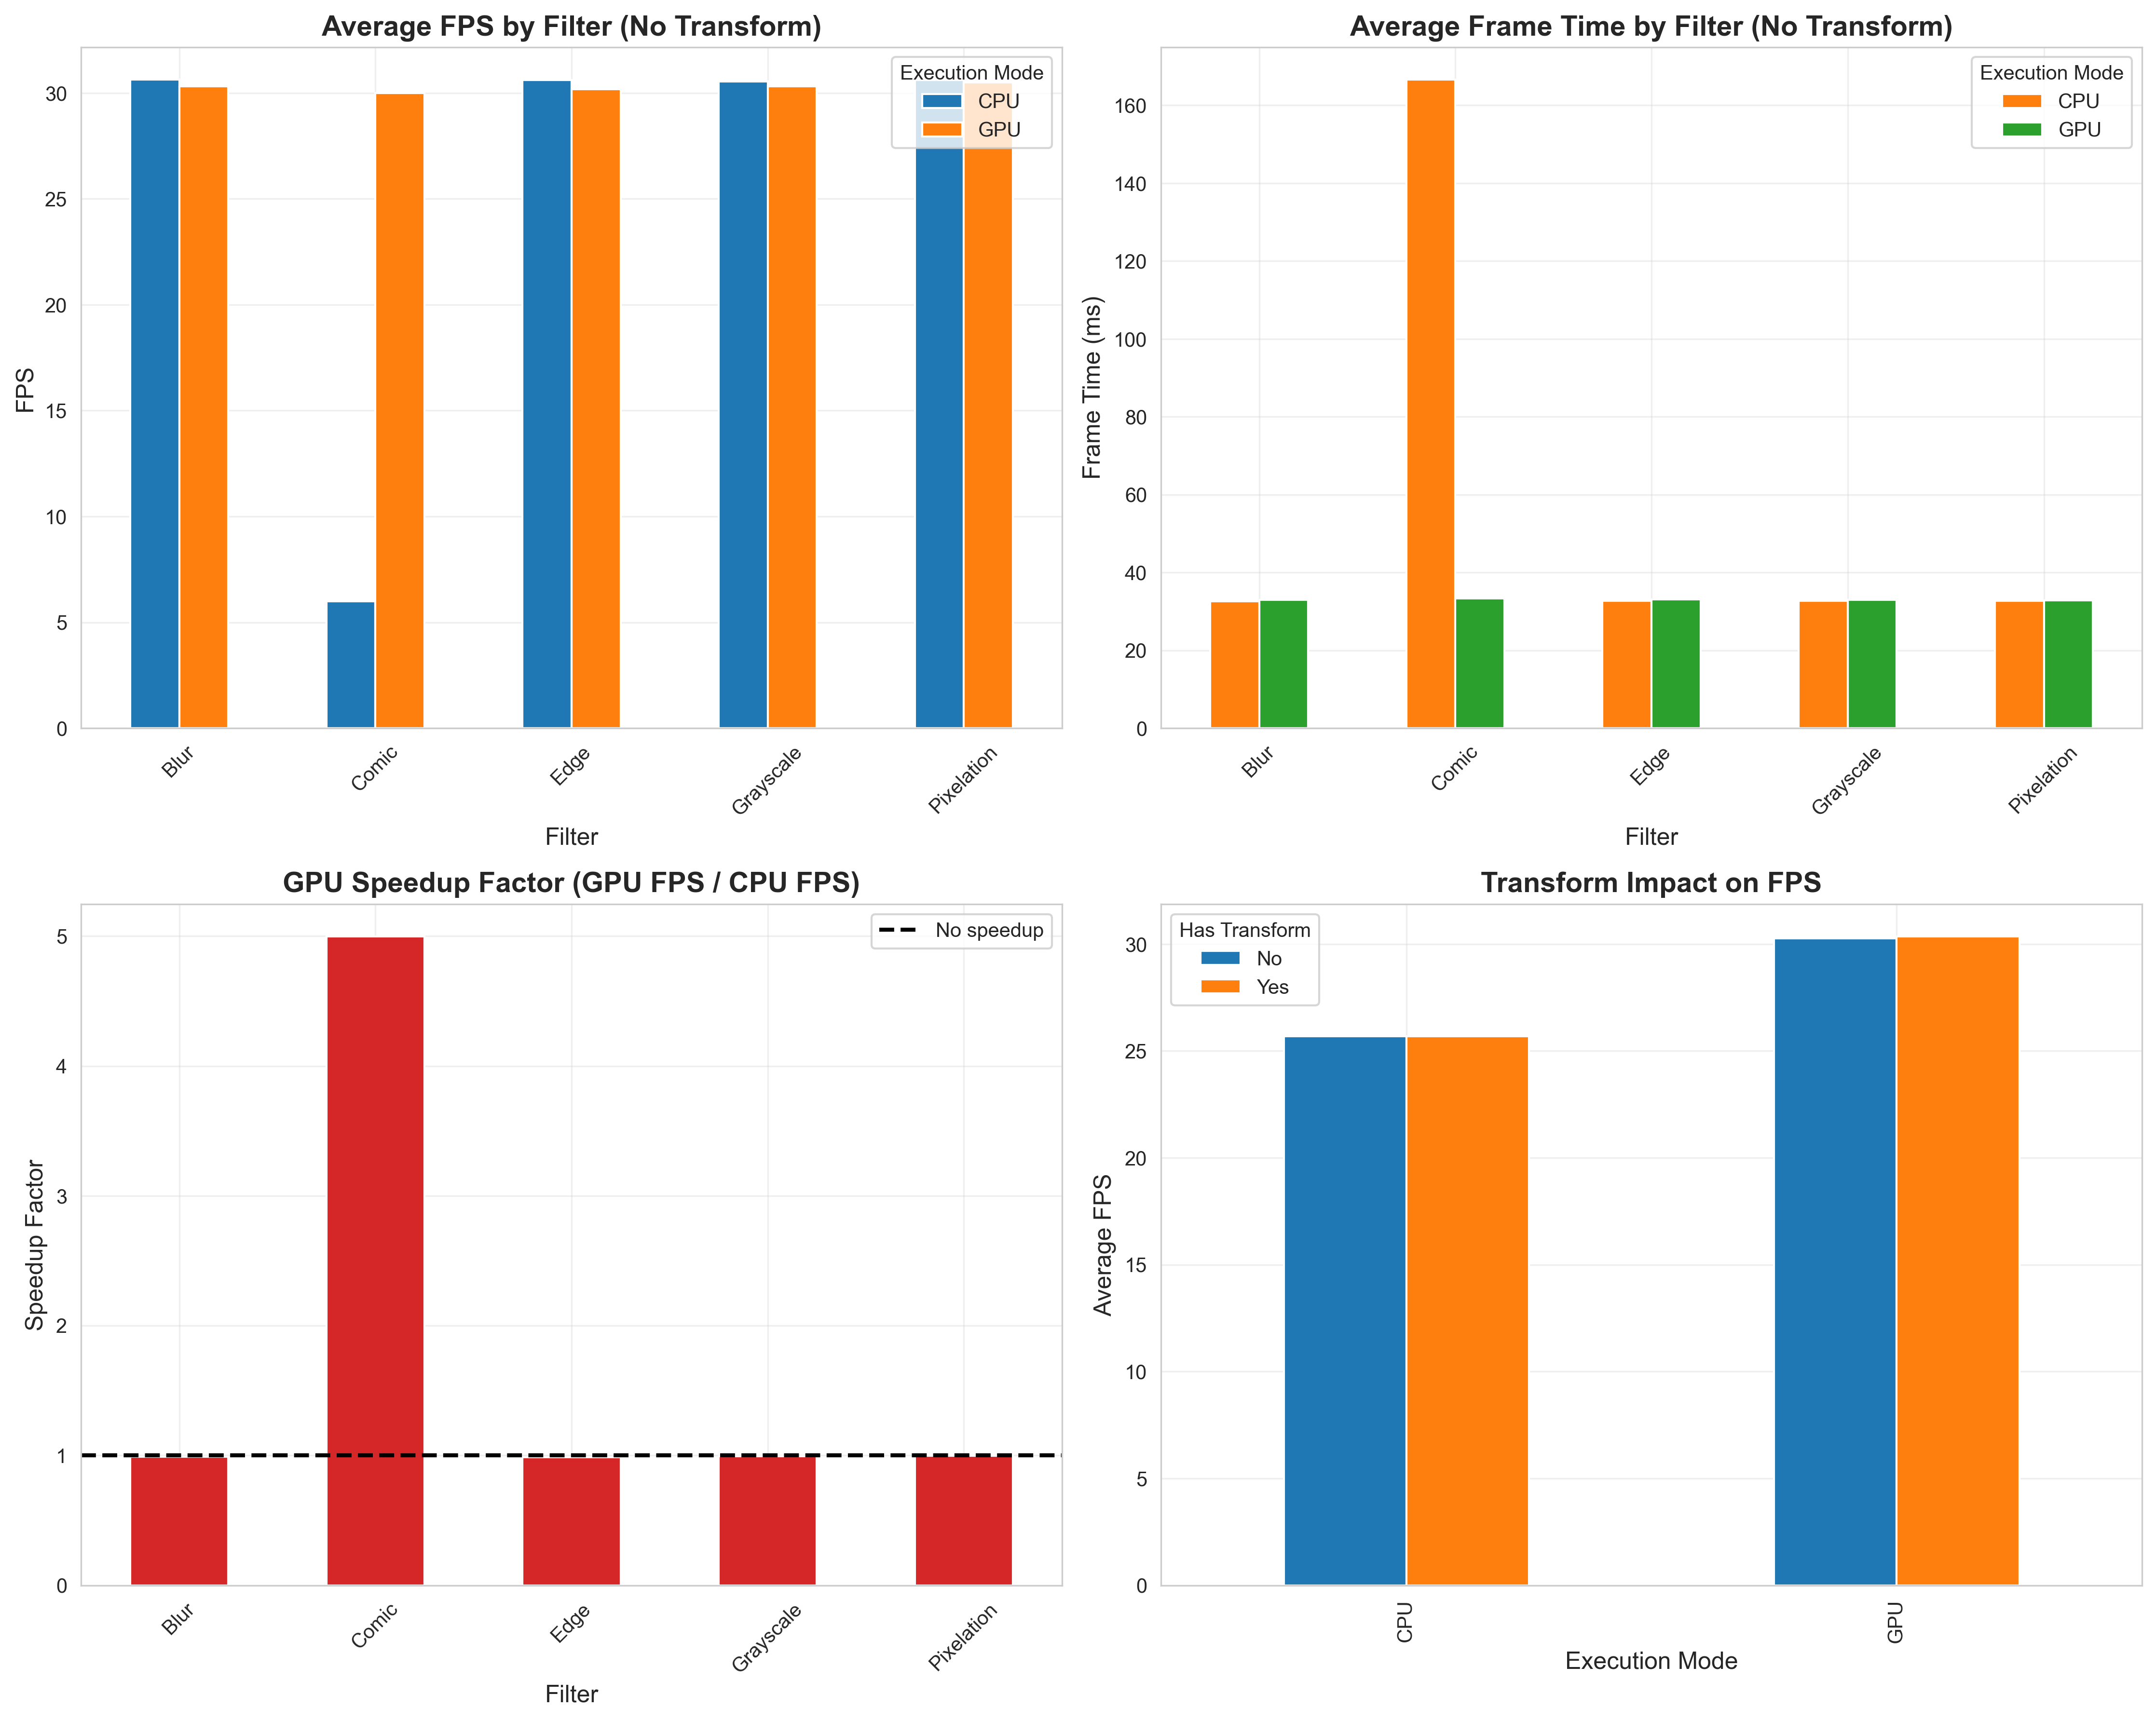
\includegraphics[width=0.75\textwidth]{../data/plots/performance_comparison_transforms.png}
    \caption{Performance comparison across filters and execution modes}
    \label{fig:transform_comparison}
\end{figure}

It's clear that the GPU outperforms the CPU significantly only for the Comic Art filter, while for all other filters the performance is roughly equivalent, with the CPU even slightly outperforming the GPU in some cases. This suggests that for simple filters, the overhead of data transfer to the GPU negates any computational advantages.

\subsubsection{Transform Impact}

\begin{figure}[H]
    \centering
    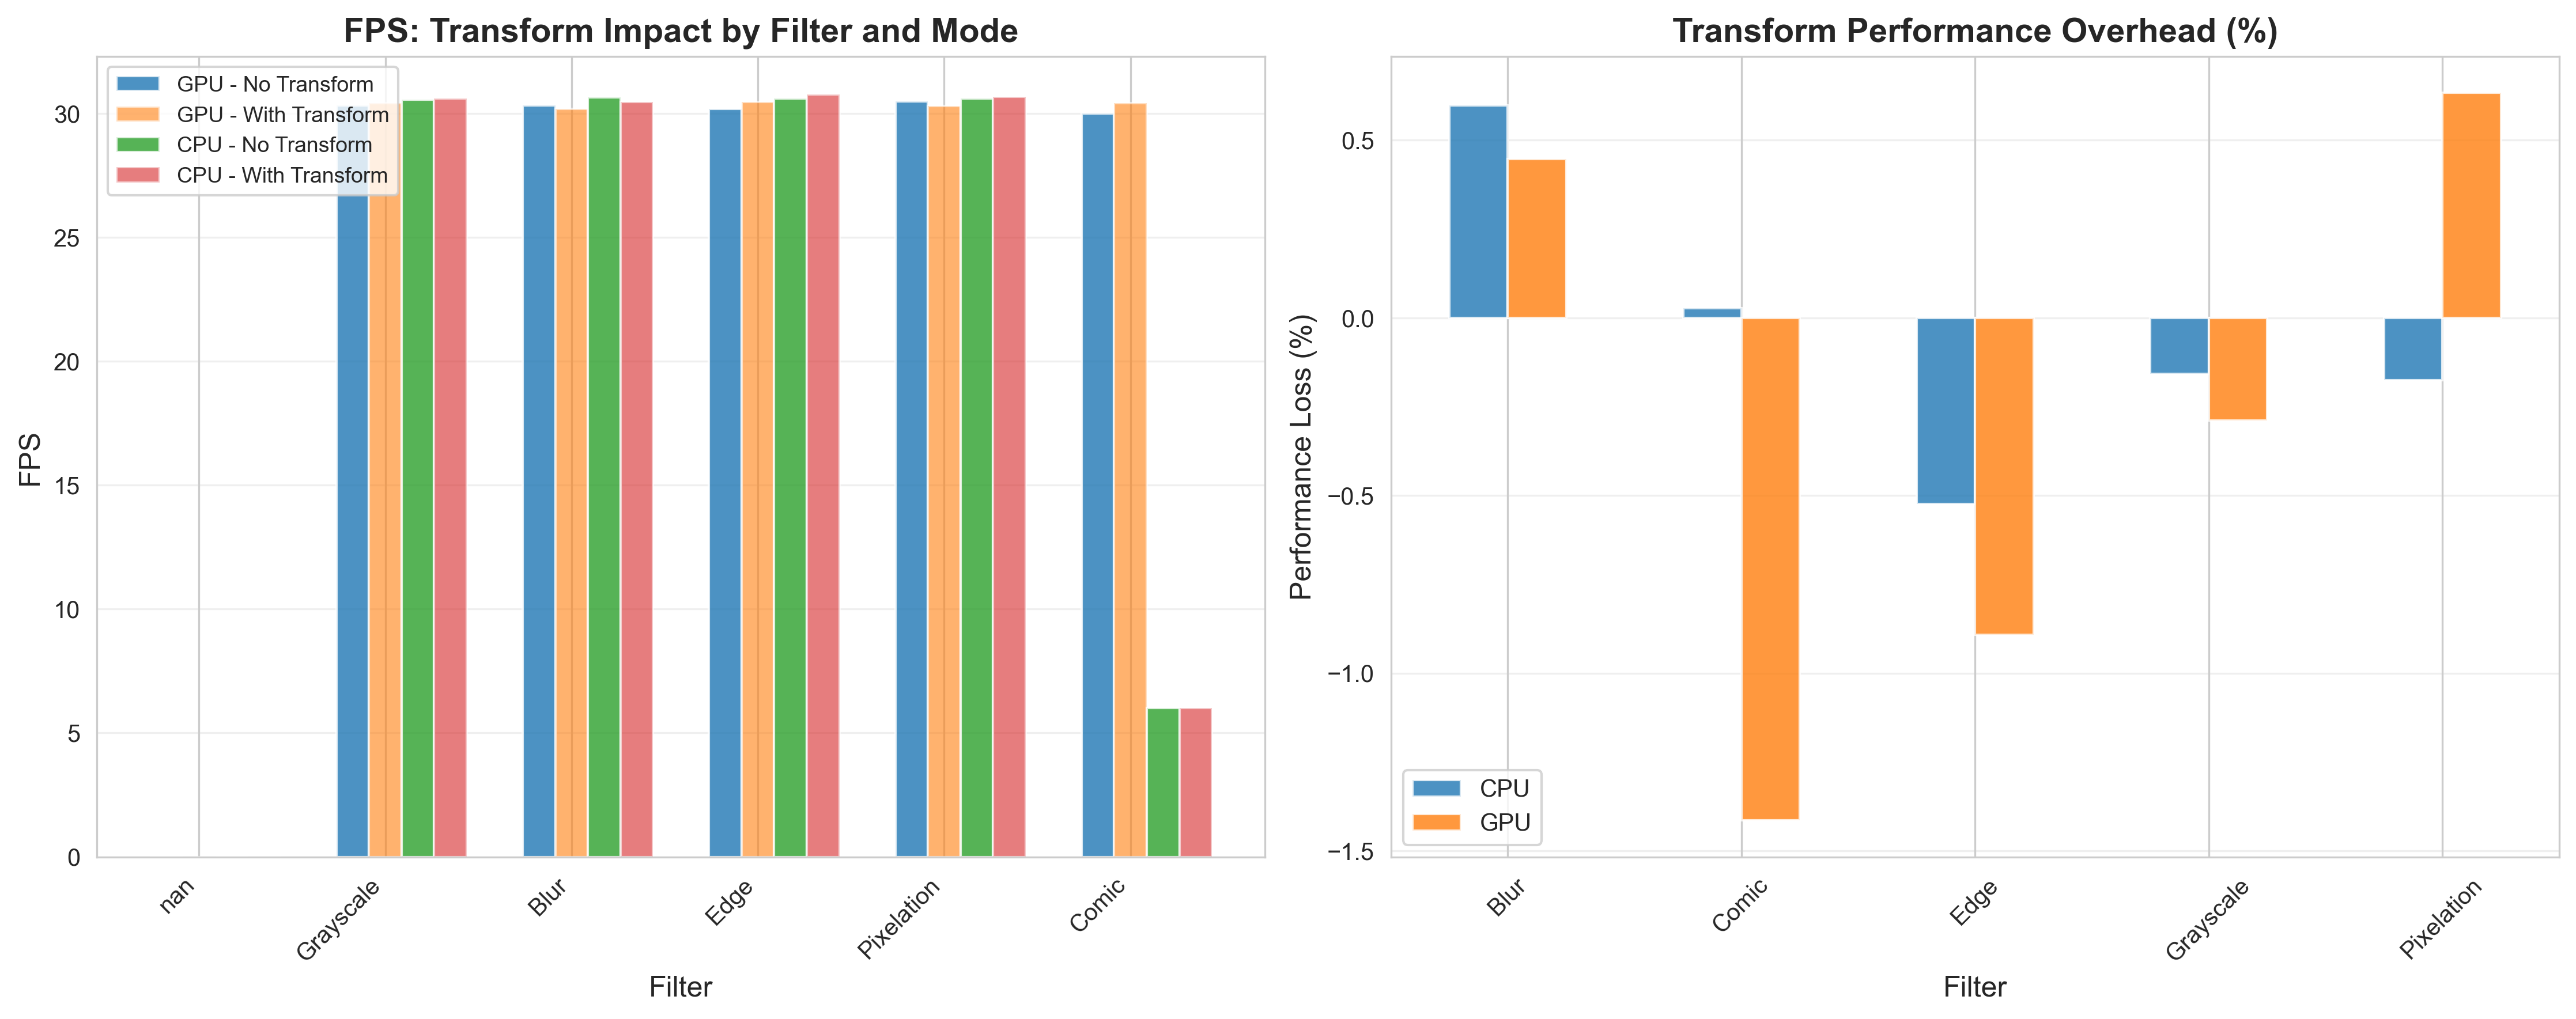
\includegraphics[width=0.75\textwidth]{../data/plots/transform_comparison.png}
    \caption{Impact of geometric transformations on performance}
    \label{fig:transform_impact}
\end{figure}

The results indicate that geometric transformations introduce minimal overhead on the GPU, with performance remaining nearly constant across all transform configurations. In contrast, CPU performance shows a slight decrease with transformations, likely due to the additional per-pixel computations required.

\subsection{Resolution Benchmark Results}

\subsubsection{Resolution Scaling}
\begin{figure}[H]
    \centering
    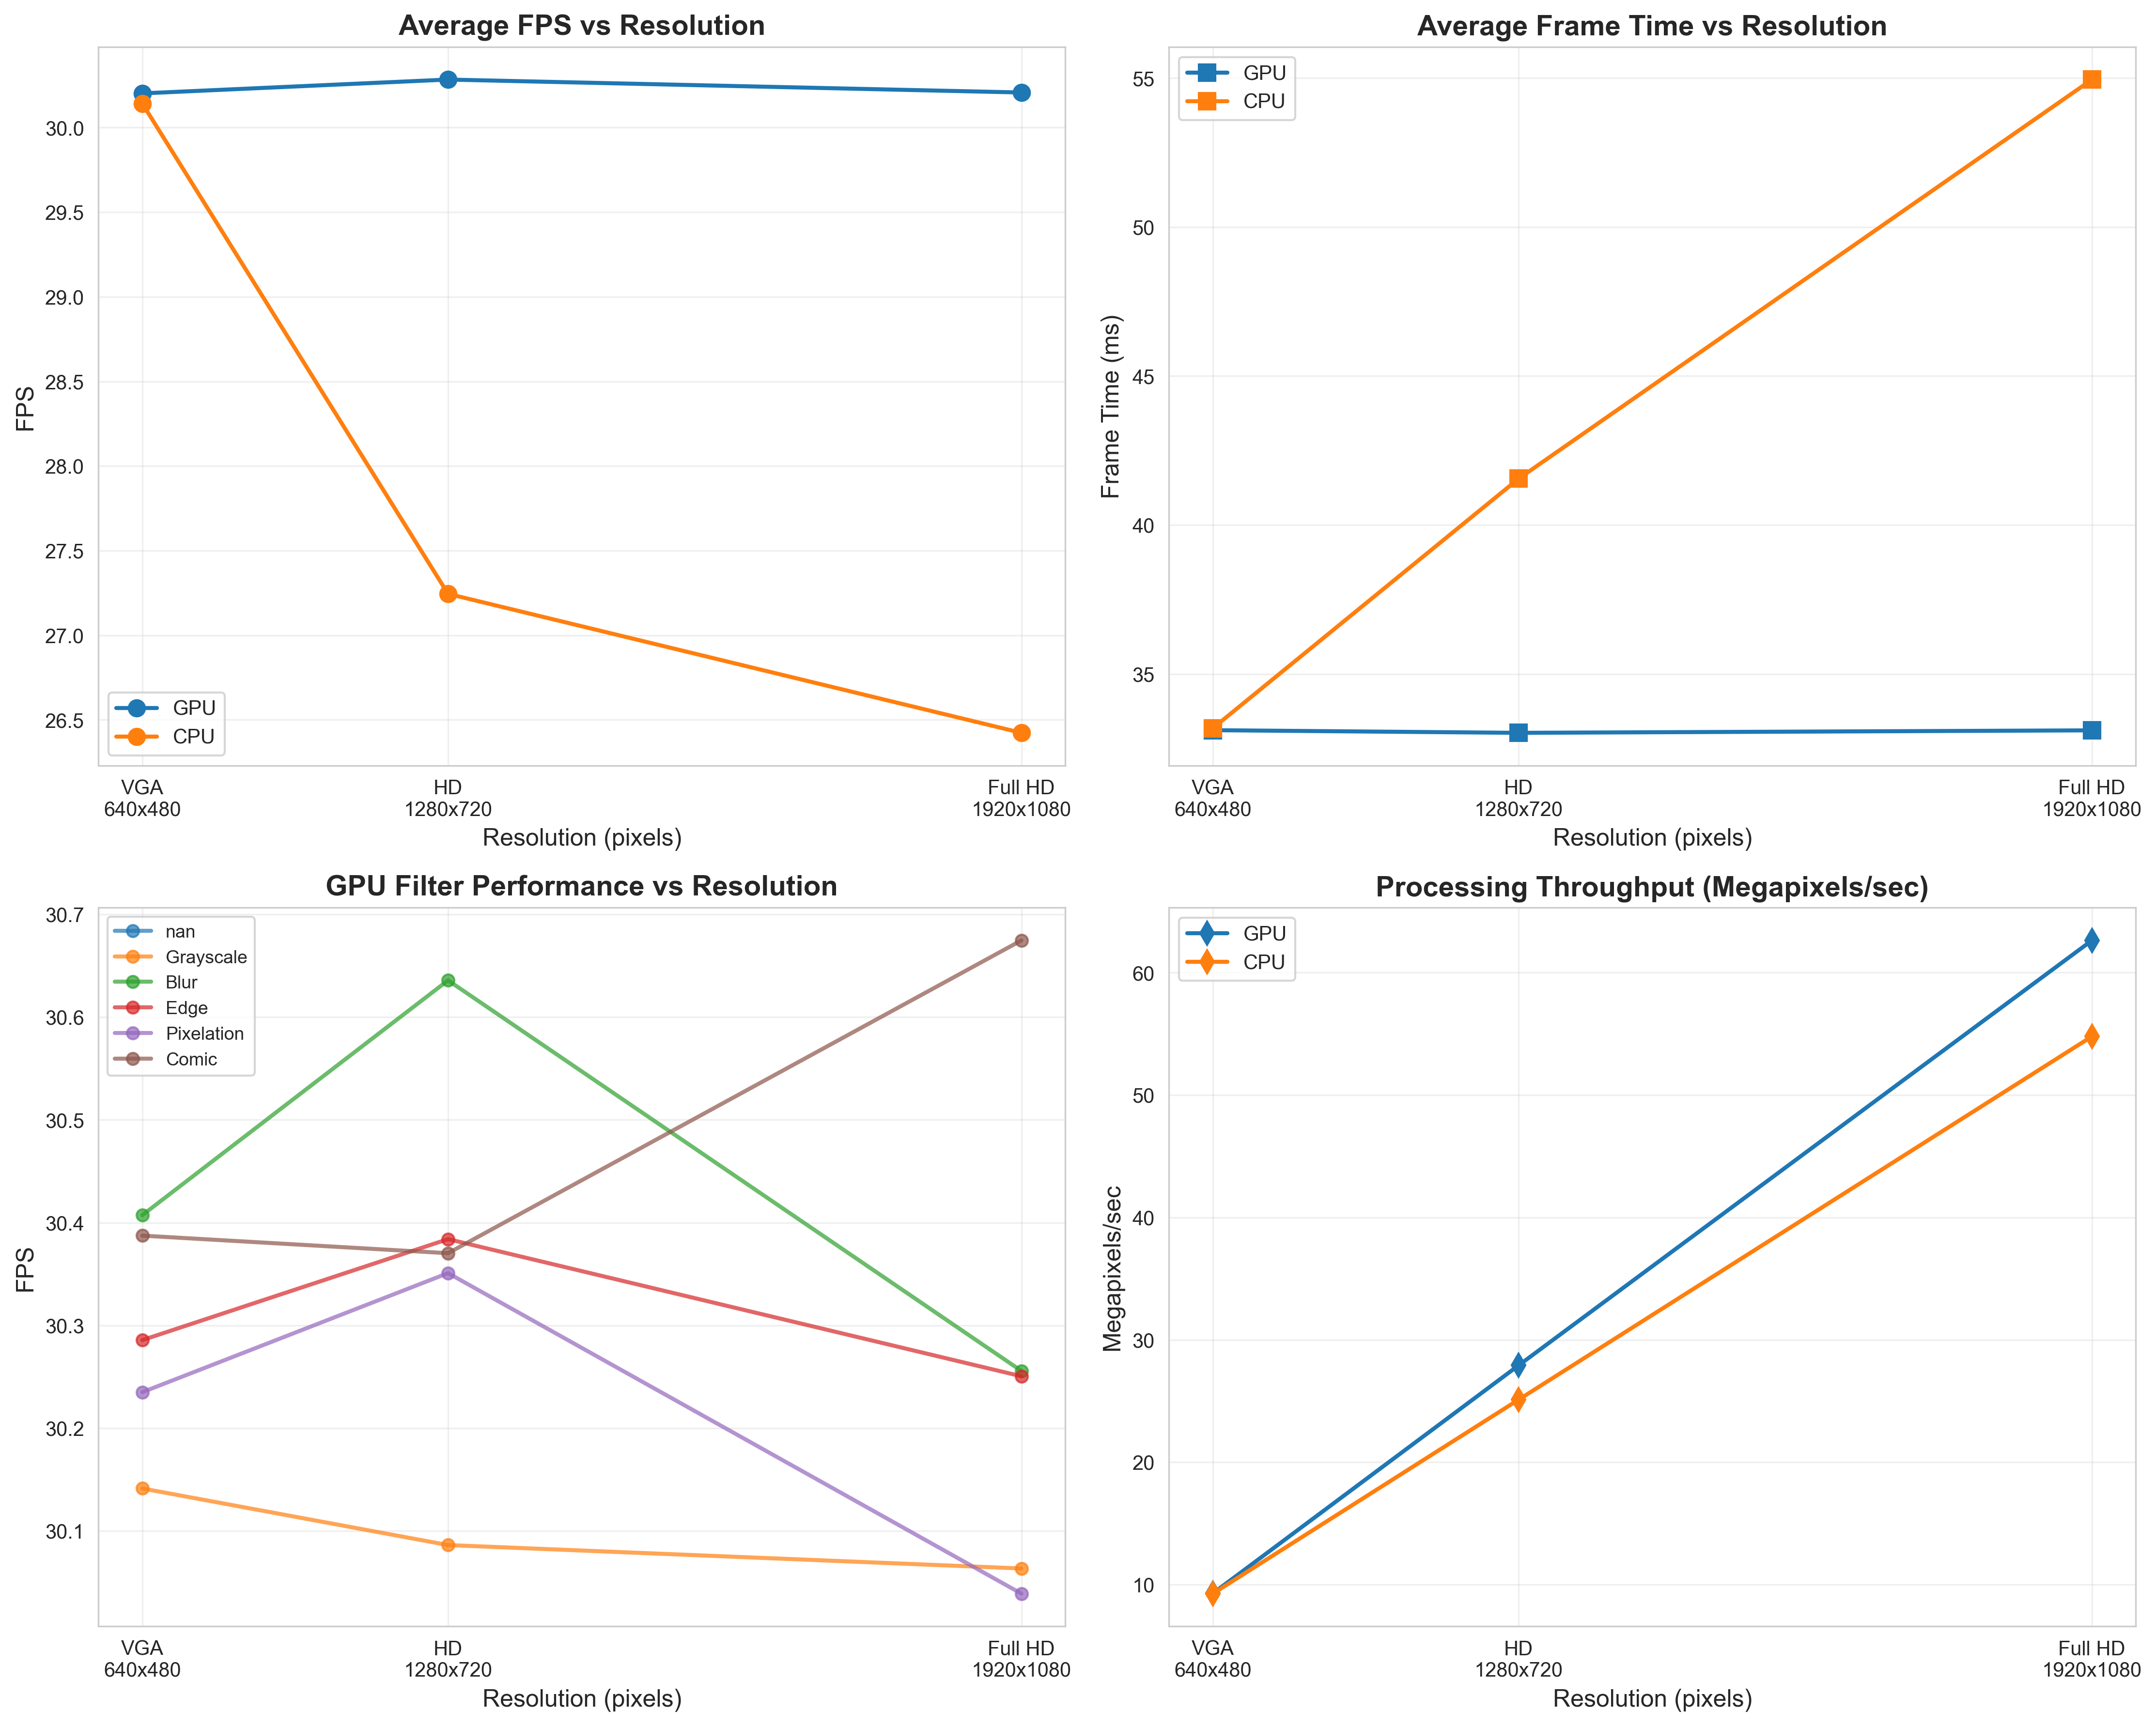
\includegraphics[width=0.6\textwidth]{../data/plots/resolution_impact.png}
    \caption{Performance across different resolutions}
    \label{fig:resolution_impact}
\end{figure}
As resolution increases, CPU performance degrades more significantly than GPU performance. The GPU maintains a relatively stable FPS across resolutions, while the CPU shows a marked decrease, highlighting the advantages of parallel processing for larger data sets.

\subsection{Performance Tables}

\begin{wraptable}{r}{0.45\textwidth}
    \centering
    \caption{GPU Speedup Factors (Resolution Tests)}
    \label{tab:speedup_resolution}
    \begin{tabular}{lc}
        \toprule
        \textbf{Filter} & \textbf{Speedup} \\
        \toprule
        None & 1.00× \\
        Grayscale & 0.99× \\
        Blur & 0.98× \\
        Edge Detection & 0.99× \\
        Pixelation & 0.99× \\
        Comic Art & \textbf{5.06×} \\
        \bottomrule
    \end{tabular}
\end{wraptable}

GPU speedup factors reveal a striking pattern: only the Comic Art filter shows meaningful performance gains on GPU (approximately 5× speedup), while all other filters demonstrate near-parity or slight CPU advantages. Speedup values less than 1.0 indicate that the CPU actually outperforms the GPU for these operations.

The resolution benchmark (Table \ref{tab:speedup_resolution}) tested filters across VGA, HD, and Full HD resolutions without geometric transformations. Results show consistent patterns across all resolutions, with simple filters achieving 0.98-0.99× speedup factors, meaning the GPU is actually 1-2\% slower than CPU due to memory transfer overhead.

\begin{wraptable}{r}{0.45\textwidth}
    \centering
    \caption{GPU Speedup Factors (Transform Tests)}
    \label{tab:speedup_transforms}
    \begin{tabular}{lc}
        \toprule
        \textbf{Filter} & \textbf{Speedup} \\
        \toprule
        None & 1.00× \\
        Grayscale & 0.99× \\
        Blur & 0.99× \\
        Edge Detection & 0.99× \\
        Pixelation & 1.00× \\
        Comic Art & \textbf{5.00×} \\
        \bottomrule
    \end{tabular}
\end{wraptable}

The transform benchmark (Table \ref{tab:speedup_transforms}) tested the same filters with five different geometric transformation configurations (none, translation, scale, rotation, combined). The results are nearly identical to the resolution benchmark, indicating that geometric transformations have minimal impact on relative performance between CPU and GPU architectures.

\section{Analysis and Discussion}
The most striking finding is that GPU processing shows no advantage for most filters, and actually performs slightly worse in some cases (Tables \ref{tab:speedup_resolution} and \ref{tab:speedup_transforms}). Only the Comic Art filter achieves meaningful GPU acceleration (~5×), while simple filters achieve 0.98-0.99× speedup factors, indicating the CPU outperforms the GPU by 1-2\%.
\\
This unexpected result likely stems from three critical factors. First, memory transfer overhead dominates processing time for simple operations. Each frame requires uploading several megabytes from system RAM to GPU memory via \texttt{glTexImage2D()}, and at Full HD resolution (2,073,600 pixels), this transfer cost exceeds the computational savings from GPU parallelism. Second, the simple filters (grayscale, blur, edge detection) impose minimal computational load. The M4 Pro's 16-core CPU with SIMD optimizations handles these operations efficiently without requiring GPU parallelism. Third, the webcam's 30 FPS limit creates a performance ceiling that prevents either architecture from demonstrating its full capability.
\\
The Comic Art filter breaks this pattern because it combines multiple operations (edge detection + color quantization) in a single GPU pass, paying off the transfer overhead across more computation. This reveals the threshold where GPU acceleration becomes beneficial: when computational complexity significantly exceeds data transfer costs. As shown in Table \ref{tab:shader_cpu_comparison}, the CPU avoids synchronization overhead and keeps data in RAM, while the GPU must transfer data every frame and synchronize via \texttt{glfwSwapBuffers()}, introducing 1-3ms latency per frame.

\subsection{Filter Complexity}
All filters except Comic Art maintain similar performance (~30 FPS on both CPU and GPU), revealing that the camera capture rate acts as the primary bottleneck rather than processing capability. Simple filters (grayscale, blur, edge detection, pixelation) fail to stress either processing architecture at typical webcam frame rates, resulting in near-identical performance regardless of execution mode. Only the Comic Art filter, with its multi-stage processing pipeline combining edge detection and color quantization, introduces sufficient computational complexity to expose meaningful differences between CPU and GPU architectures, making it the most revealing filter for understanding when GPU acceleration becomes advantageous.

\subsection{Resolution Impact}
CPU performance degrades more than GPU as resolution increases from VGA to Full HD (Figure \ref{fig:resolution_impact}). GPU parallelism scales better with the 6.75× pixel increase, though transfer overhead still limits absolute performance gains.

\subsubsection{Implications}
The results suggest that for higher resolutions, GPU processing becomes more advantageous due to its ability to handle larger data sets more efficiently through parallelism. This is especially true for more complex filters, where the computational load is higher. 

\subsection{Transform Overhead}

Geometric transformations reveal a stark architectural difference between GPU and CPU processing. GPU transformations operate exclusively in the vertex shader, applying mathematical operations to just 4 vertices per frame regardless of resolution. The GPU's dedicated vertex processors handle rotation, scaling, and translation trivially, with no measurable FPS impact between transformed and non-transformed rendering. This efficiency stems from the fact that transformations occur before rasterization, affecting only the corner coordinates of the quad that holds the video texture.
\\
In contrast, CPU transformations using OpenCV's \texttt{warpAffine()} function must process every pixel individually. The function performs interpolation calculations across the entire frame, typically using bilinear or bicubic methods to determine pixel values at fractional coordinates. This per-pixel processing creates less cache-friendly memory access patterns compared to sequential filter operations, as the transformation requires sampling from non-contiguous memory locations based on the inverse transformation matrix.
\\
Despite these architectural disadvantages, CPU transform overhead remains minimal in practice, introducing only 1-2\% FPS reduction as shown in Figure \ref{fig:transform_impact}. Three factors contribute to this surprisingly small impact: the webcam's 30 FPS framerate cap limits overall throughput regardless of processing method, OpenCV's highly optimized implementation leverages SIMD instructions and efficient memory management, and the tested transformations are simple affine operations (not complex perspective warps or non-linear distortions) that allow for optimized code paths. The results demonstrate that while GPU vertex shaders are theoretically superior for geometric operations, the practical performance difference becomes negligible when constrained by camera hardware limitations.

\subsection{GPU Pipeline Architecture and Bottlenecks}

The GPU pipeline uses GLSL 3.3 shaders: vertex shaders apply transformations to 4 vertices using 2D rotation matrices, while fragment shaders process all pixels in parallel. Six fragment shaders implement the filters (Table \ref{tab:filters}).

\begin{table}[H]
\centering
\caption{GPU Pipeline Bottlenecks}
\label{tab:gpu_bottlenecks}
\begin{tabular}{lp{7cm}}
\toprule
\textbf{Bottleneck} & \textbf{Impact} \\
\midrule
Texture Upload & \texttt{glTexImage2D()} transfers several MB per frame (RAM → GPU). At Full HD, transfer time exceeds simple filter processing time. \\
Synchronization & \texttt{glfwSwapBuffers()} adds some latency per frame. CPU avoids this entirely. \\
Memory Bandwidth & Convolution filters require 9-25 texture samples per pixel, stressing GPU cache and memory subsystems. \\
\bottomrule
\end{tabular}
\end{table}
Table \ref{tab:shader_cpu_comparison} shows why CPU wins for simple filters: data stays in RAM, no synchronization overhead, and SIMD-optimized OpenCV functions are highly efficient. GPU advantages only emerge when computational complexity (Comic Art) exceeds the transfer cost across multiple operations.
\begin{table}[H]
\centering
\caption{GPU vs CPU Implementation Differences}
\label{tab:shader_cpu_comparison}
\begin{tabular}{lll}
\toprule
\textbf{Aspect} & \textbf{GPU} & \textbf{CPU} \\
\midrule
Data Transfer & Every frame & Stays in RAM \\
Synchronization & 1-3 ms/frame & None \\
Parallelism & Massive & Limited \\
Transform Cost & 4 vertices & All pixels \\
\bottomrule
\end{tabular}
\end{table}

\subsubsection{Conclusion}
This investigation reveals that GPU acceleration is not universally superior for real-time video processing. Data transfer costs between system RAM and GPU memory can exceed the computational gains from parallelism, particularly for simple operations like grayscale conversion or basic blurring. GPU advantages only emerge when computational complexity is sufficient to pay off the transfer overhead, as demonstrated by the Comic Art filter's 5× speedup through its multi-stage edge detection and color quantization pipeline. Additionally, graphics rendering pipelines optimized for rasterization are suboptimal for general image processing tasks, and camera frame rate limitations (30 FPS) create a performance ceiling that masks the true capabilities of both architectures. For typical webcam applications at standard frame rates, CPU processing with SIMD-optimized libraries like OpenCV often matches or exceeds GPU performance for all but the most complex multi-stage filters, challenging the conventional assumption that GPUs are inherently better for real-time image processing.
\subsection{Showcasing Filters}
\begin{figure}[H]
    \centering
    \begin{subfigure}[b]{0.32\textwidth}
        \centering
        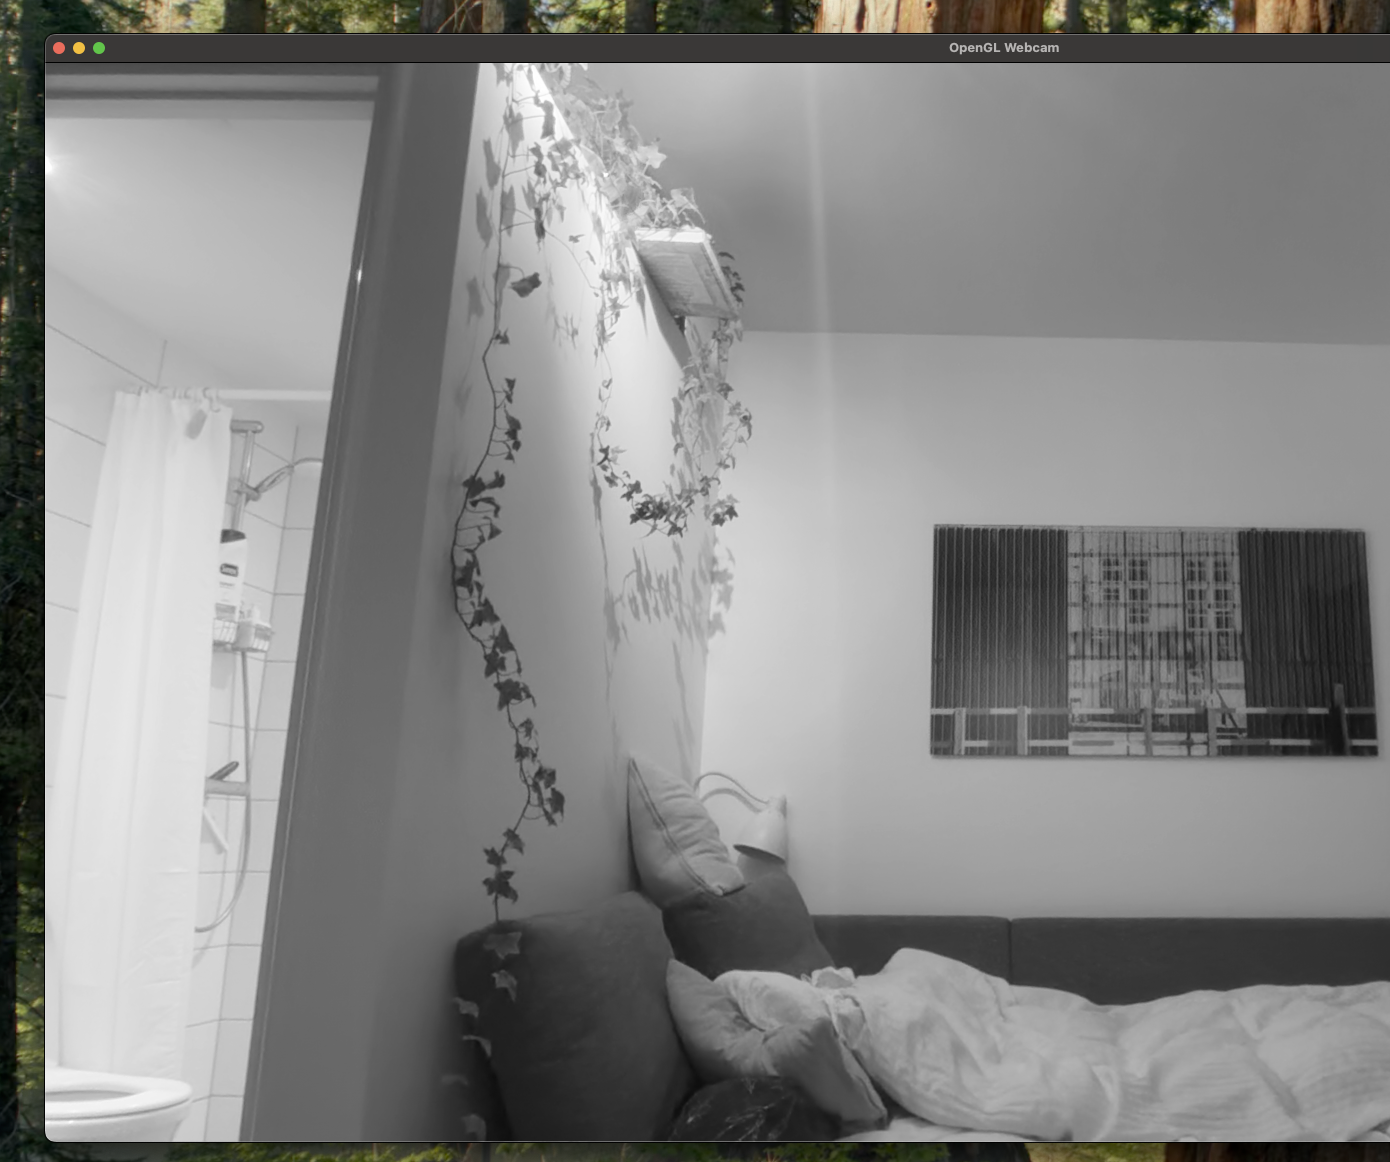
\includegraphics[width=\textwidth]{filters/grey.png}
        \caption{Grayscale}
        \label{fig:filter_grayscale}
    \end{subfigure}
    \hfill
    \begin{subfigure}[b]{0.32\textwidth}
        \centering
        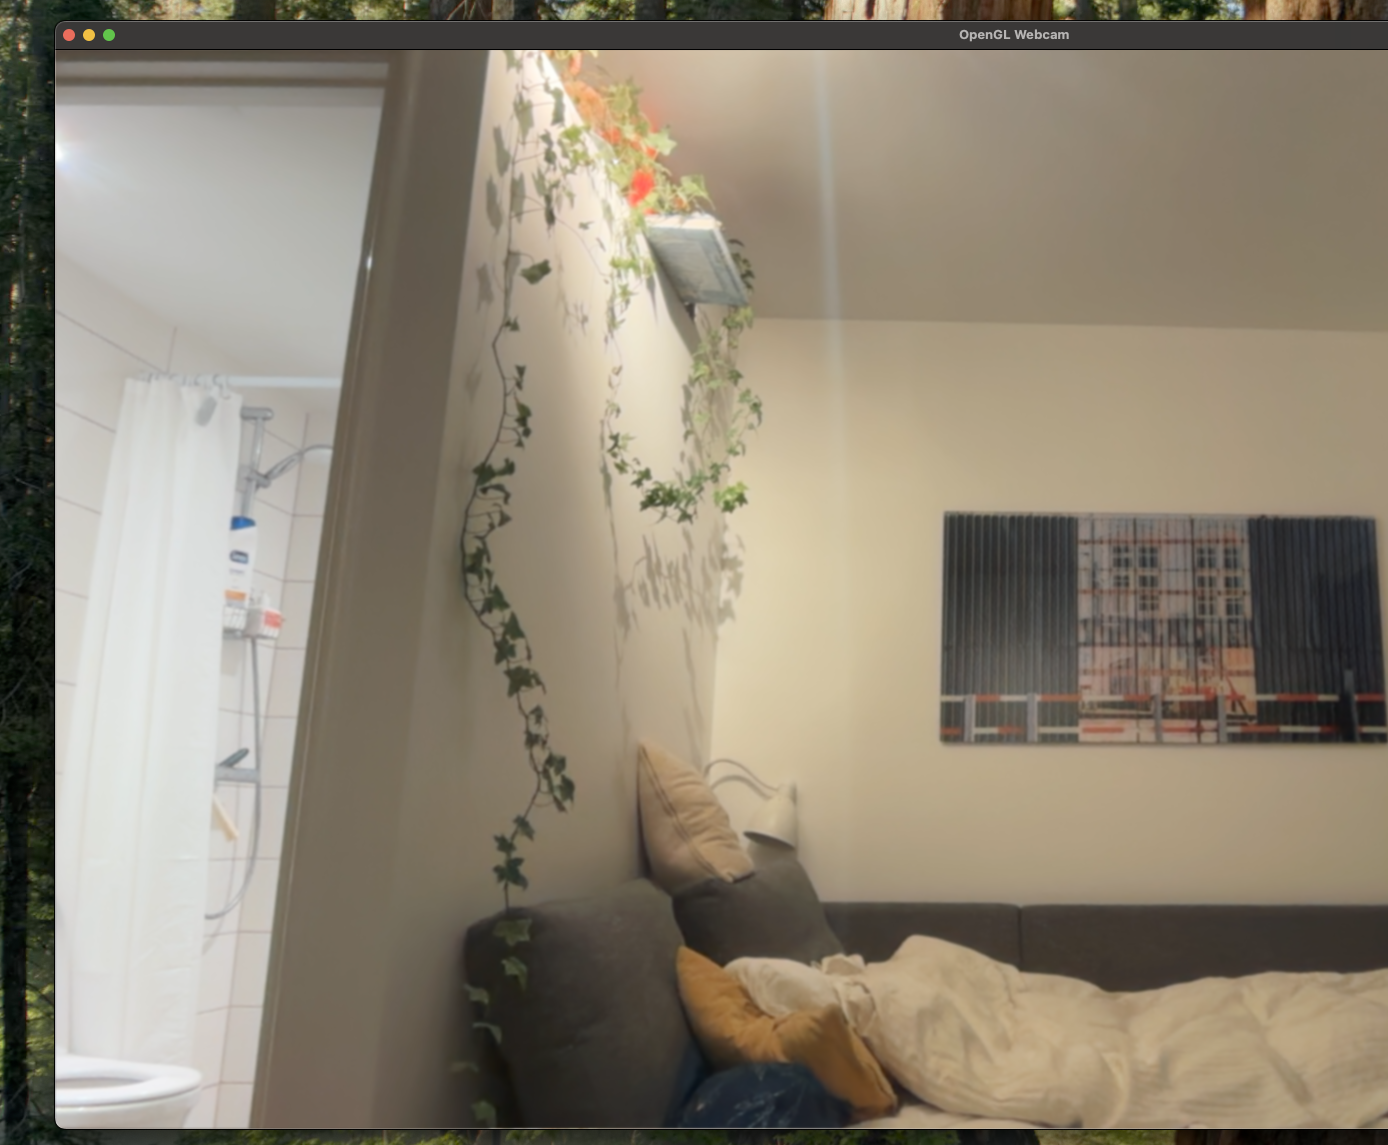
\includegraphics[width=\textwidth]{filters/gblur.png}
        \caption{Gaussian Blur}
        \label{fig:filter_blur}
    \end{subfigure}
    \hfill
    \begin{subfigure}[b]{0.32\textwidth}
        \centering
        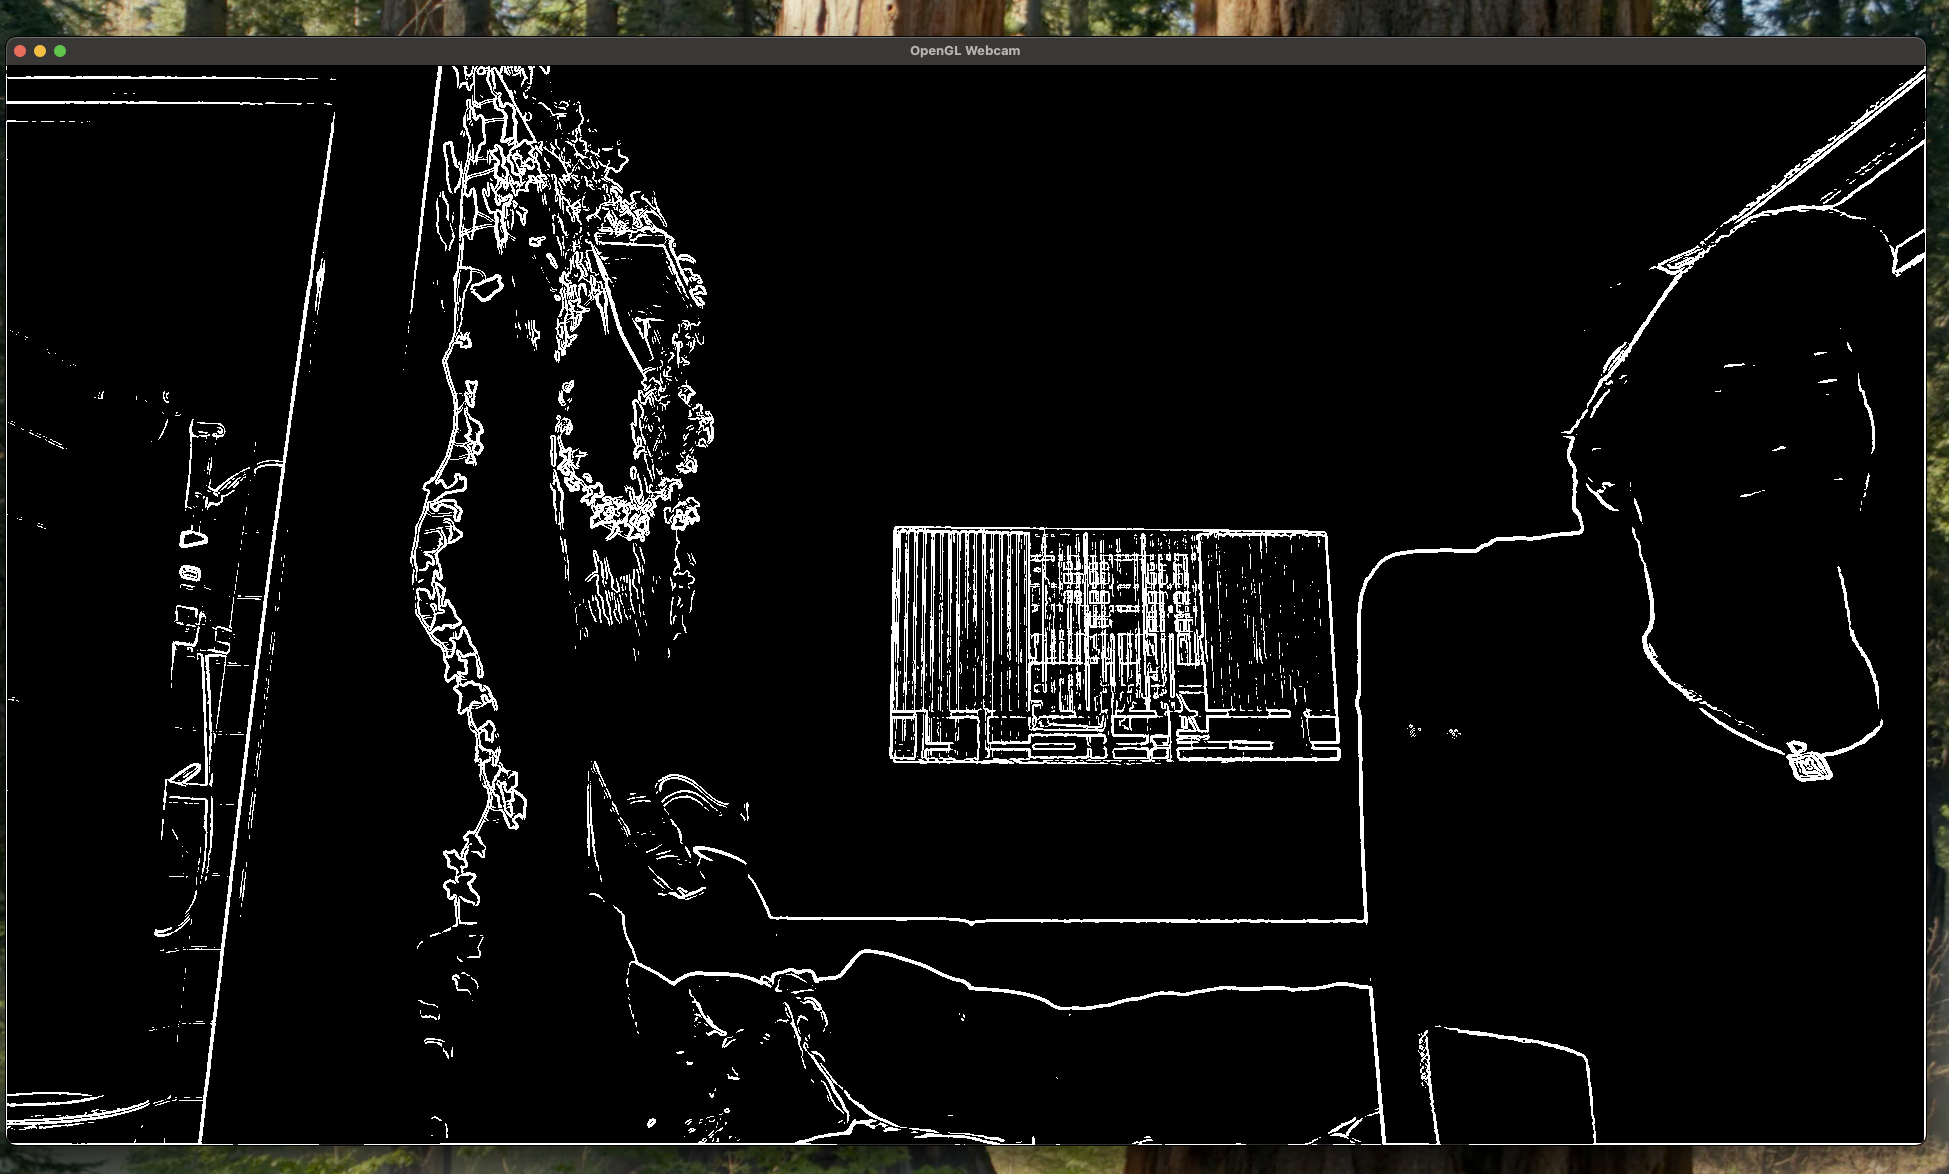
\includegraphics[width=\textwidth]{filters/edge.png}
        \caption{Edge Detection}
        \label{fig:filter_edge}
    \end{subfigure}
    
    \vspace{0.5cm}
    
    \begin{subfigure}[b]{0.32\textwidth}
        \centering
        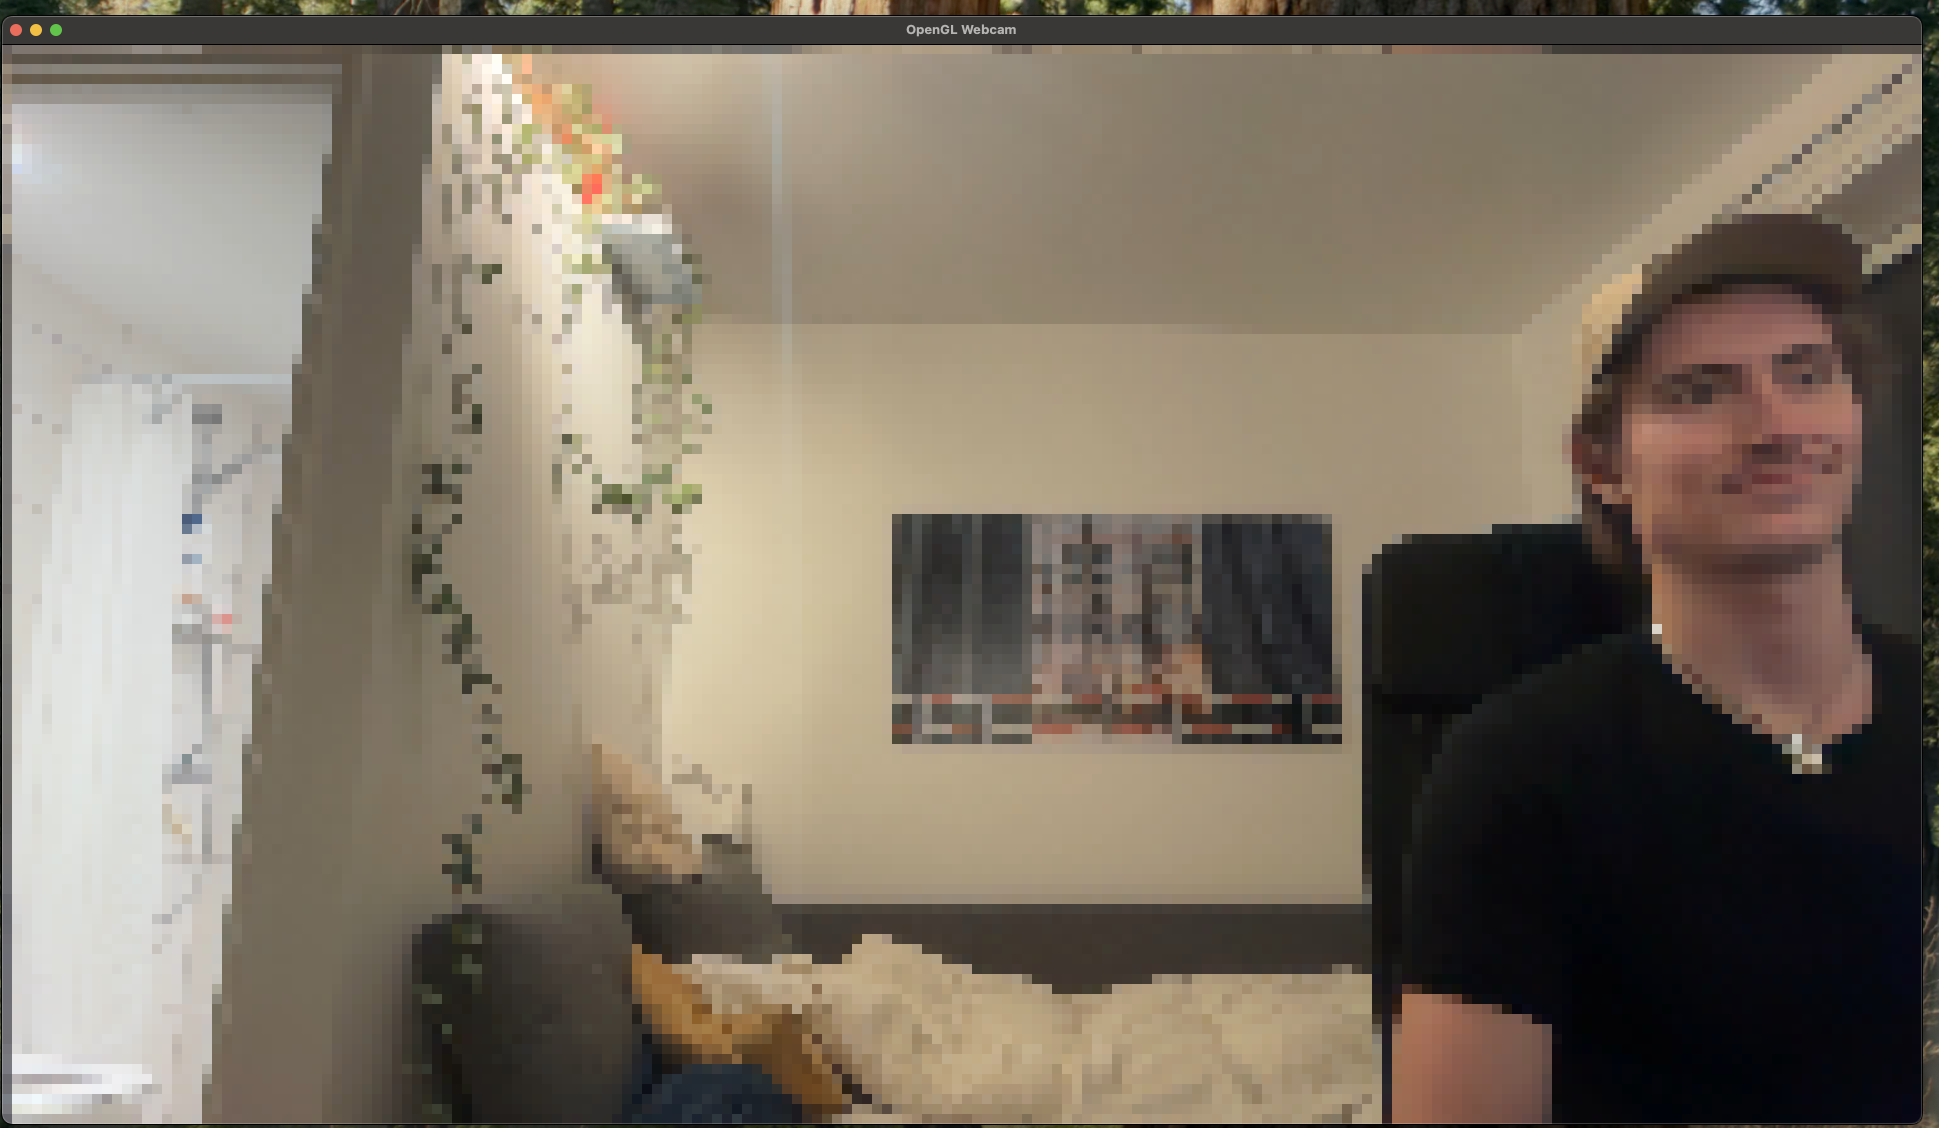
\includegraphics[width=\textwidth]{filters/pixelatio.png}
        \caption{Pixelation}
        \label{fig:filter_pixelation}
    \end{subfigure}
    \hfill
    \begin{subfigure}[b]{0.32\textwidth}
        \centering
        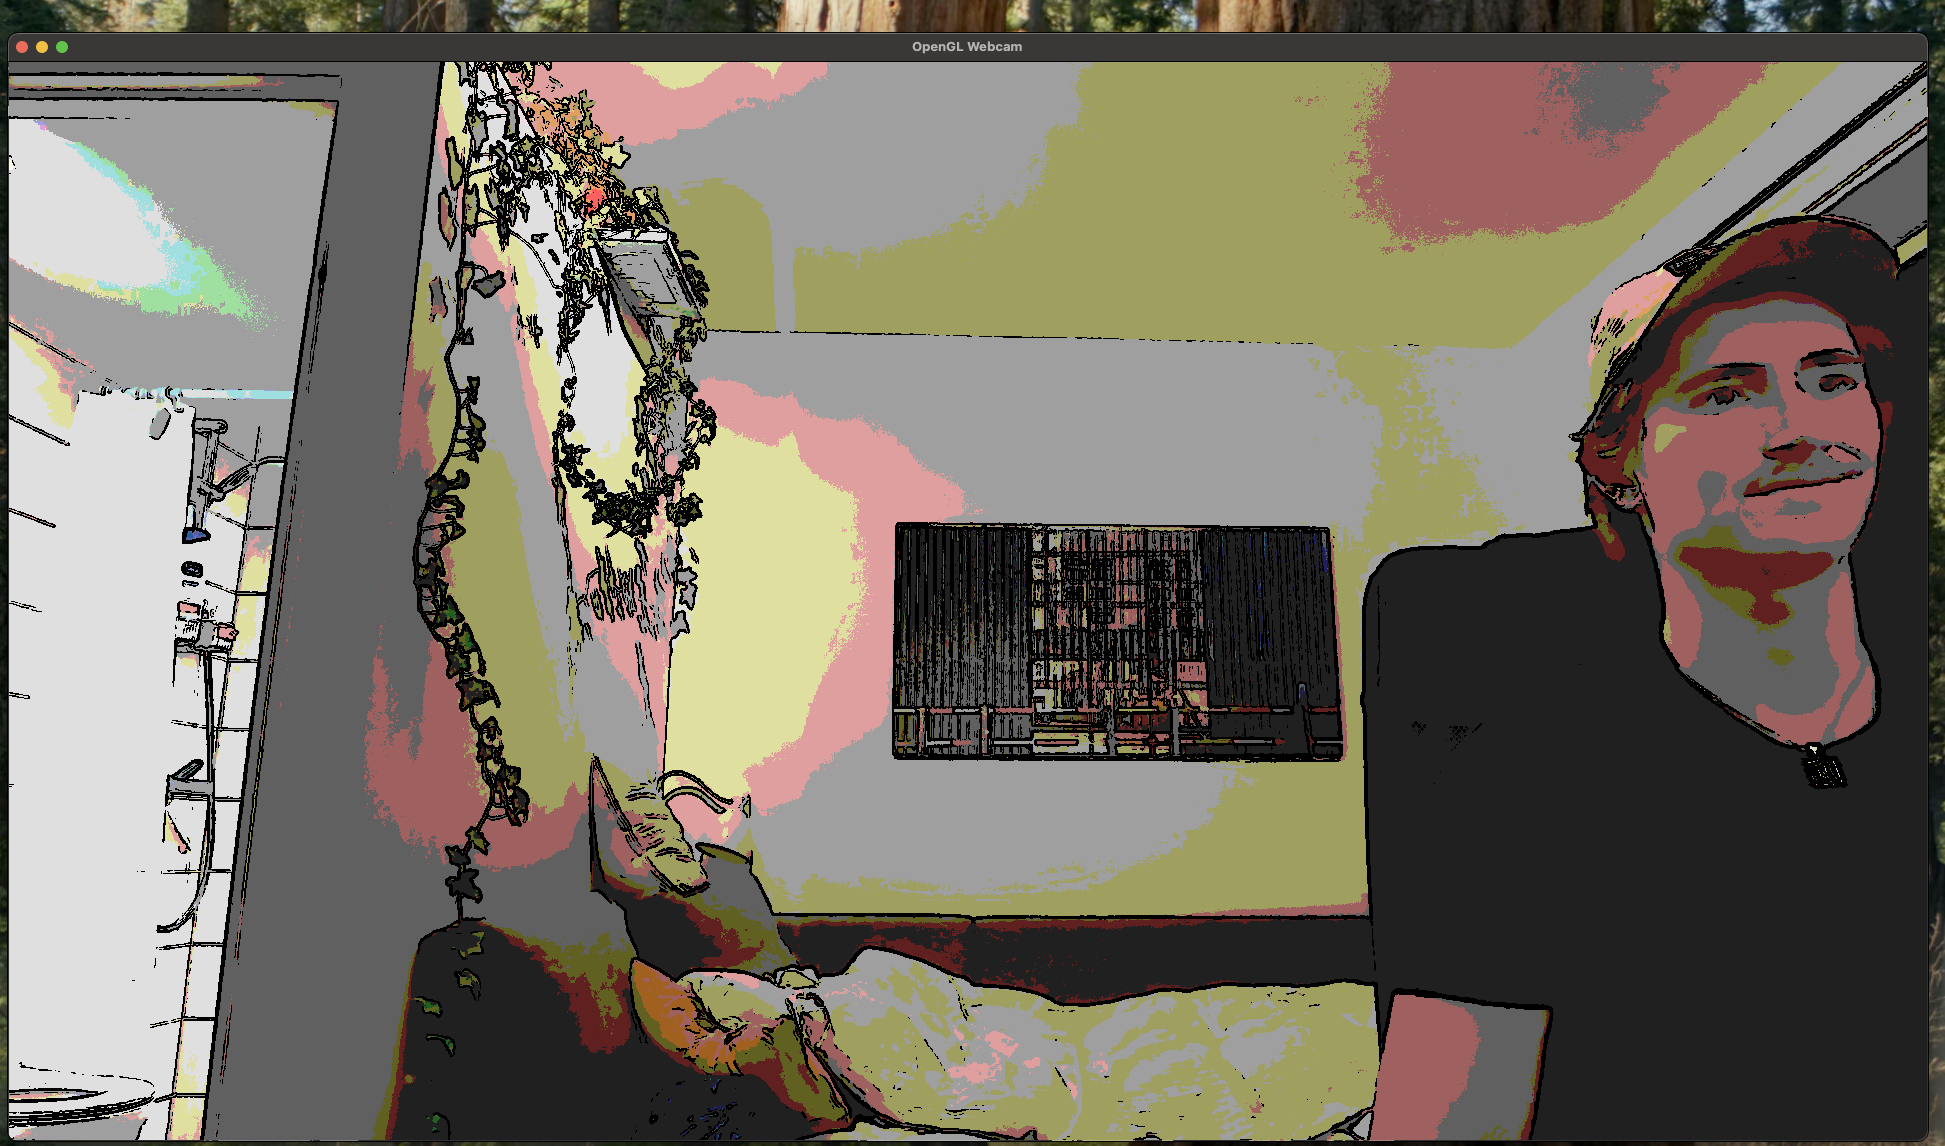
\includegraphics[width=\textwidth]{filters/comic.png}
        \caption{Comic Art}
        \label{fig:filter_comic}
    \end{subfigure}

    \caption{Visual comparison of implemented filters applied to the same input frame. (a) Grayscale conversion reduces color information. (b) Gaussian blur creates smoothing effect. (c) Edge detection highlights contours using Sobel operator. (d) Pixelation creates blocky mosaic effect. (e) Comic art combines edge detection with color quantization for artistic effect.}
    \label{fig:filter_comparison}
\end{figure}


\end{document}